\section{Résultats}

\paragraph{Dimensions} Avant de commencer les essais de traction, la longueur \(L_0\), largeur \(\ell\) et épaisseur \(e\) des parties fines des échantillons ont étés mesurées. Les dimensions sont reportées dans le \autoref{tab:dims}. Les trois échantillons présentant les résultats les plus réguliers ont été conservés.

\begin{table}[h]
    \centering
    % TODO supprimer inutiles
    \begin{tabular}{ |c||c|c|c|c| }
        \cline{2-5}
        \multicolumn{1}{c|}{} & Échantillon n$^\circ$ & \(L_0\) [mm] & \(\ell\) [mm] & \(e\) \\
        \hline
        \multirow{1}{4cm}{Non-traité}
        % & 1 & \(18.13 \pm 0.01\) & \(4.21 \pm 0.01\) & \(2.30 \pm 0.01\) \\
        & 2 & \(20.46 \pm 0.01\) & \(4.19 \pm 0.01\) & \(2.07 \pm 0.01\) \\
        \hline
        \multirow{1}{4cm}{Adouci}
        & 3 & \(17.42 \pm 0.01\) & \(4.05 \pm 0.01\) & \(2.01 \pm 0.01\) \\
        % & 4 & \(17.41 \pm 0.01\) & \(4.09 \pm 0.01\) & \(2.00 \pm 0.01\) \\
        \hline
        \multirow{1}{4cm}{Adouci puis durci}
        % & 5 & \(18.04 \pm 0.01\) & \(4.06 \pm 0.01\) & \(2.03 \pm 0.01\) \\
        & 6 & \(18.19 \pm 0.01\) & \(4.12 \pm 0.01\) & \(2.04 \pm 0.01\) \\
        % & 7 & \(18.81 \pm 0.01\) & \(4.20 \pm 0.01\) & \(2.04 \pm 0.01\) \\
        \hline
    \end{tabular}
    \caption{Dimensions des échantillons avant la traction}
    \label{tab:dims}
\end{table}

\paragraph{Essais de traction}
Il a bien été observé empiriquement pour tous les essais de traction effectués dans l'ordre: une déformation élastique, une déformation plastique suivie d'une striction puis d'une rupture. Une figure pour chaque traitement thermique est donnée en \autoref{fig:tractions_exp} montrant l'extraction du module de Young $E$, de la contrainte maximale $\sigma_\mathrm{max}$ et de la déformation rémanente à la rupture $\varepsilon_{\textrm{rup}}$. La limite élastique $\sigma_{0.2}$ est aussi indiquée.
% L'ensemble des figures restantes avec les annotations sont disponibles en \autoref{sec:fig_supp}.
Les valeurs de la limite élastique $\sigma_{0.2}$ ont été déterminées comme illustré en \autoref{fig:limite_elastique} où les figures correspondantes pour deux échantillons sélectionnés sont disponibles. Toutes ces valeurs ont été prélevées selon la théorie présentée en \autoref{sec:theorie} et en utilisant le module de Young obtenu précédement pour chaque essai de traction. Les valeurs numériques correspondantes sont dans le \autoref{tab:results}.

Une comparaison entre les courbes de traction des échantillons traités et non traité se trouve en \autoref{fig:comparaison}.

\begin{figure}[h!]
    \centering
    \begin{subfigure}{0.48\linewidth}
        \centering
        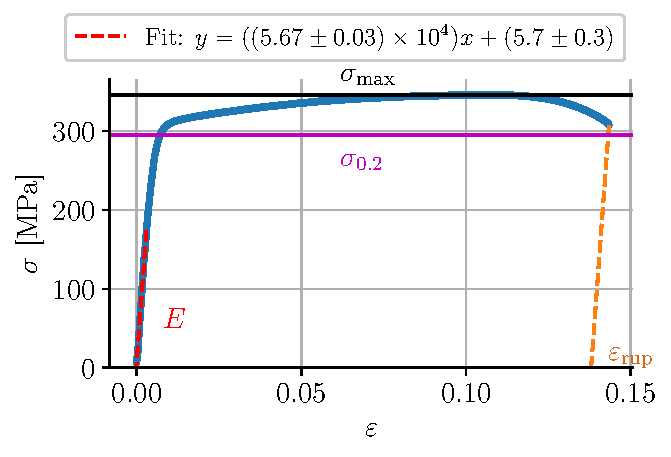
\includegraphics[width=\linewidth]{figures/froid2all.pdf}
        \caption{}
        \label{fig:froid2}
    \end{subfigure}
    \begin{subfigure}{0.48\linewidth}
        \centering
        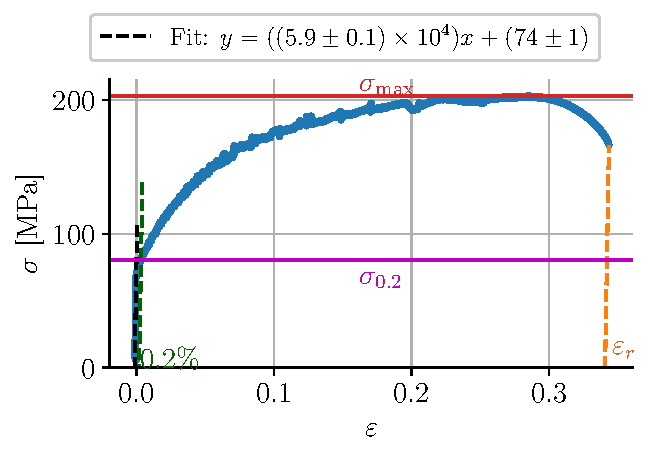
\includegraphics[width=\linewidth]{figures/chaud3all.pdf}
        \caption{}
        \label{fig:chaud3}
    \end{subfigure}
    \begin{subfigure}{0.48\linewidth}
        \centering
        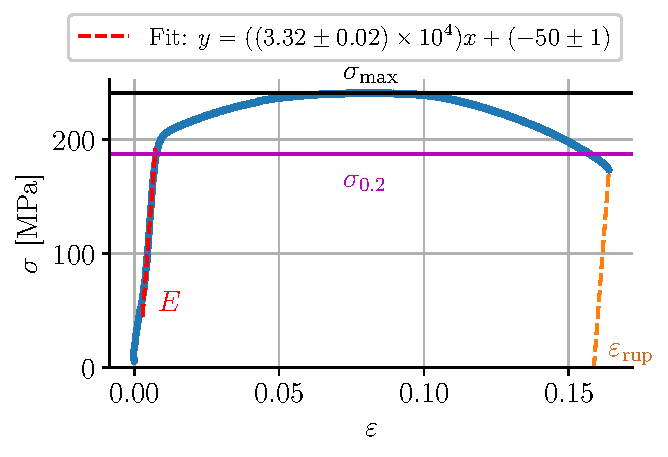
\includegraphics[width=\linewidth]{figures/tiede6all.pdf}
        \caption{}
        \label{fig:tiede6}
    \end{subfigure}
    \begin{subfigure}{0.48\linewidth}
        \centering
        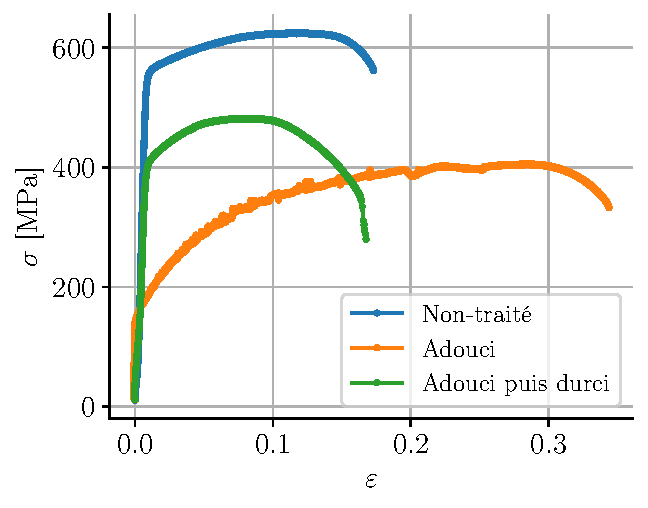
\includegraphics[width=\linewidth]{figures/comparaison.pdf}
        \caption{}
        \label{fig:comparaison}
    \end{subfigure}
    \caption{Courbe de traction pour un échantillon (a) non-traité (b) adouci (c) adouci puis durci. Une régression linéaire a été réalisée afin d'obtenir le module de Young \(E\) permettant de déterminer \(\sigma_{0.2}\) et \(\varepsilon_{\textrm{rup}}\). En (d) une comparaison entre les courbes de traction obtenues pour des échantillons non traité, adouci et adouci puis durci}
    \label{fig:tractions_exp}
\end{figure}

\begin{figure}[H]
    \centering
    \begin{subfigure}{0.48\linewidth}
        \centering
        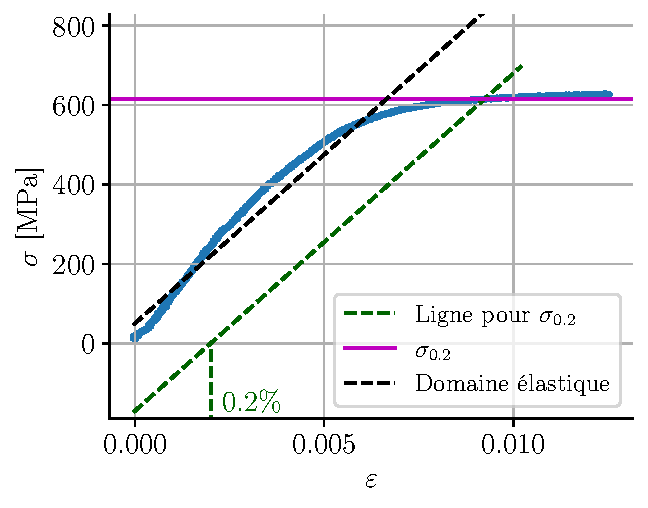
\includegraphics[width=\linewidth]{figures/froid2_sigma2.pdf}
        \caption{}
        \label{fig:froid1_lim}
    \end{subfigure}
    \begin{subfigure}{0.48\linewidth}
        \centering
        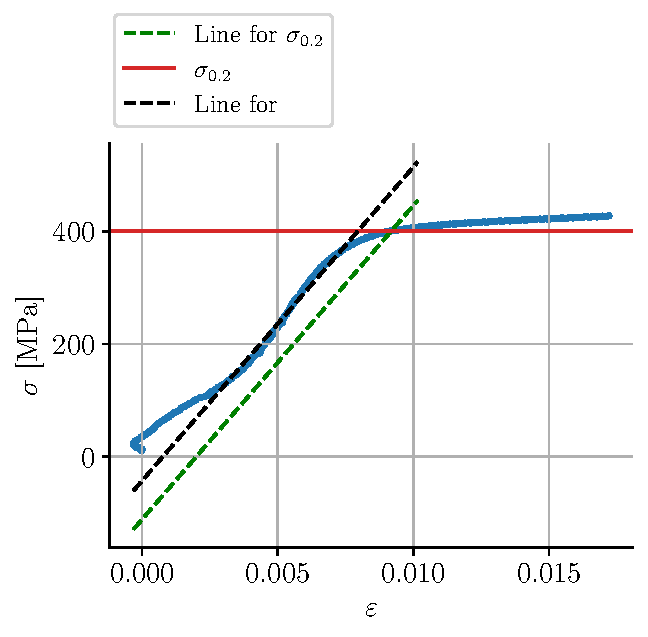
\includegraphics[width=\linewidth]{figures/tiede6_sigma2.pdf}
        \caption{}
        \label{fig:tiede6_lim}
    \end{subfigure}
    \caption{Extraction de la limite élastique $\sigma_{0.2}$ en connaissant le module de Young $E$ pour un échantillon (a) non-traité (b) adouci puis durci}
    \label{fig:limite_elastique}
\end{figure}


\begin{table}[h]
    \centering
    \begin{tabular}{ |c||c|c|c|c|c| }
        \cline{2-6}
        \multicolumn{1}{c|}{} & Échantillon n$^\circ$ & \(E\) [GPa] & \(\sigma_{0.2}\) [MPa] & \(\sigma_{\textrm{max}}\) [MPa] & \(\varepsilon_{\textrm{rup}}\) [\%] \\
        \hline
        \multirow{1}{4cm}{Non-traité}
        % & 1 & \input{data/froid1_E} & \input{data/froid1_sigma2} & \input{data/froid1_s_max} & \input{data/froid1_eps_rup} \\
        & 2 & \input{data/froid2_E} & \input{data/froid2_sigma2} & \input{data/froid2_s_max} & \input{data/froid2_eps_rup} \\
        \hline
        \multirow{1}{4cm}{Adouci}
        & 3 & \input{data/chaud3_E} & \input{data/chaud3_sigma2} & \input{data/chaud3_s_max} & \input{data/chaud3_eps_rup} \\
        % & 4 & \input{data/chaud4_E} & \input{data/chaud4_sigma2} & \input{data/chaud4_s_max} & \input{data/chaud4_eps_rup} \\
        \hline
        \multirow{1}{4cm}{Adouci puis durci}
        % & 5 & \input{data/tiede5_E} & \input{data/tiede5_sigma2} & \input{data/tiede5_s_max} & \input{data/tiede5_eps_rup} \\
        & 6 & \input{data/tiede6_E} & \input{data/tiede6_sigma2} & \input{data/tiede6_s_max} & \input{data/tiede6_eps_rup} \\
        % & 7 & \input{data/tiede7_E} & \input{data/tiede7_sigma2} & \input{data/tiede7_s_max} & \input{data/tiede7_eps_rup} \\
        \hline
    \end{tabular}
    \caption{Module de Young \(E\), limite élastique \(\sigma_{0.2}\), résistance à la traction \(\sigma_{\textrm{max}}\) et déformation à la rupture \(\varepsilon_{\textrm{rup}}\) pour les échantillons non-traités, adoucis et adoucis puis durcis}
    \label{tab:results}
\end{table}

Les résultats obtenus pour l'échantillon non-traité ont été comparés aux valeurs tabulées de l'alliage d'aluminium 6061-T6, dont la composition est la plus proche de l'Anticorodal 110 \cite{alualualu}. La comparaison est dans le \autoref{tab:err_rel}.

\begin{table}[h]
    \centering
    \begin{tabular}{ |c||c|c|c|c| }
        \cline{2-5}
        \multicolumn{1}{c|}{} & \(E\) [GPa] & \(\sigma_{0.2}\) [MPa] & \(\sigma_{\textrm{max}}\) [MPa] & \(\varepsilon_{\textrm{rup}}\) [\%] \\
        \hline
        \multirow{1}{4cm}{Valeur de référence}
        & 69 & 275 & 310 & \(\ge\)12 \\
        \hline
        \multirow{1}{4cm}{Erreur relative}
        & \input{data/froid2_E_rel}\% & \input{data/froid2_sigma2_rel}\% & \input{data/froid2_s_max_rel}\% & \input{data/froid2_eps_rup_rel}\% \\
        \hline
    \end{tabular}
    \caption{Comparaison entre l'échantillon non-traité et les valeurs tabulées pour l'alliage 6061-T6 \cite{alualualu}}
    \label{tab:err_rel}
\end{table}

